\subsubsection{Klassifikation af KOLs sværhedsgrad}
Ved diagnose af KOL inddeles patienterne i klassifikationer. Dette vurderes på baggrund af patienternes symptomer, egne erfaringer og vurderinger i forhold til livskvalitet. Hertil anvendes Medical Research Council åndenødsskala (MRC) og COPD assessment test (CAT) til klassificering.\cite{Basisbogen2016}
 
MRC-skalaen er en skala fra $1$-$5$, hvor patienten vurderer mængden af aktivitet, der kan udføres i forhold til åndenød, der opleves. Skalaen fremgår af \autoref{fig:MRC}, hvor $1$ svarer til, at patienten først oplever åndenød ved meget anstrengelse, og $5$ svarer til, at patienten oplever åndenød ved meget lav aktivitet. \cite{Basisbogen2016}

\begin{figure} [H]
\centering
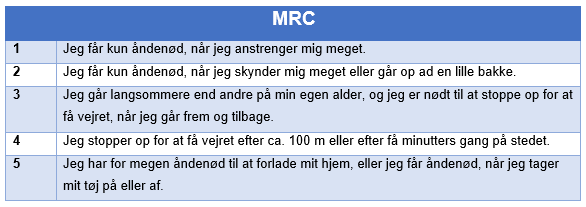
\includegraphics[width=1\textwidth]{figures/MRC}
\caption{MRC-skala som viser skalaen fra $1$-$5$. Patienter der oplever åndenød ved meget anstrengelse kategoriseres som $1$, mens patienter der oplever åndenød ved lav aktivitet kategoriseres som $5$.}
\label{fig:MRC}
\end{figure} 

\noindent
Ud fra MRC-skalaen, lungefunktionstest og antallet af eksacerbationer det seneste år opnås CAT-scoren. Derudover vurderes det på baggrund af patientens egne vurderinger af symptomer, såsom slim i lungerne, hoste og åndenød. Patienten vurderer symptomerne fra $0$ til $5$, hvormed $0$ vurderes til at patienten ingen symptomer har. Jo højere den samlede score er, desto værre vurderes patienten symptomer. \cite{Basisbogen2016, dsam2016} Patienterne inddeles i CAT-scoren ud fra fire forskellige kategorier; A, B, C og D, hvilket fremgår af \autoref{fig:CAT}.

\begin{figure} [H]
\centering
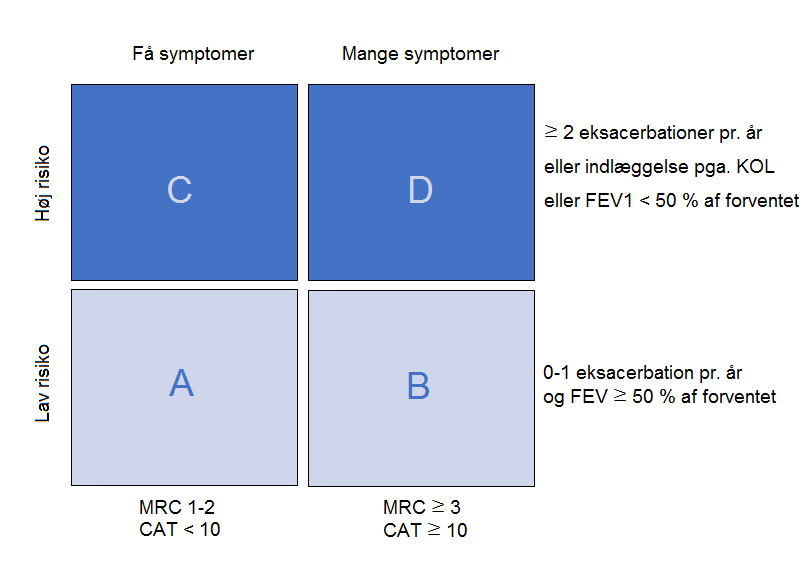
\includegraphics[width=0.8\textwidth]{figures/CAT}
\caption{CAT-scoren er inddelt i fire kategorier, herunder A, B, C og D. D kategoriceres som en patient med mange symptomer og er i høj risiko, mens patienter der kategoriseres i A oplever få symptomer og er i lav risiko.}
\label{fig:CAT}
\end{figure} 
 
\noindent
**** HER SKAL GOLD KOBLES SAMMEN MED INDDELING AF GOlD ***
*** DETTE ER EN HJEMME OPGAVE - SE UDKOMMENTERET LINK ***
% https://pro.medicin.dk/Sygdomme/Sygdom/318294 

Sværhedsgraden af KOL klassificeres af Dansk Selskab for Almen Medicin (DSAM) ud fra retningslinjer opstillet af the Global Initiative for Chronic Obstructive Lung Disease (GOLD). Disse klassificeres ud fra spirometrimålinger. 

Sværhedsgraden af KOL kan også klassificeres udelukkende ud fra spirometrimålinger. Sværhedsgraderne inddeles i fire GOLD-stadier, som kan ses af \autoref{fig:GOLD}.

\begin{figure} [H]
\centering
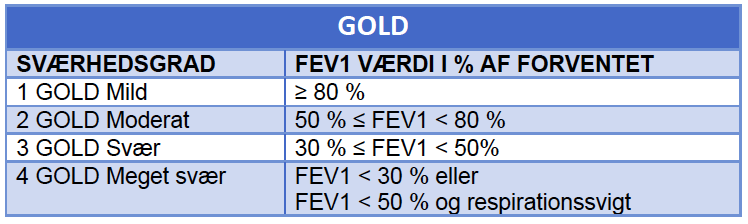
\includegraphics[width=0.8\textwidth]{figures/GOLD}
\caption{GOLD-stadier er inddelt efter sværhedsgraderne $1$-$4$ herunder mild, moderat, svær og meget svær. Patienter i 1 GOLD mild har over $80~\%$ af forventet lungekapacitet, mens patienter i 4 Meget svær har under $30~\%$ eller under $50~\%$ af forventet lungekapacitet samt respirationssvigt.}
\label{fig:GOLD}
\end{figure} 

\subsection{Behandling}
Det er ikke muligt at behandle patienter med KOL, men det er muligt at bremse udviklingen af KOL samt lindre symptomerne. Dette kan opnås ved tobakafvænning, fysisk aktivitet, kostvejledning og medicin. 

Da den tabte lungefunktionen ikke kan genvindes, rådes patienterne til rygestop hurtigst muligt for således at bibeholde den nuværende lungefunktion. Det fremgår af \autoref{fig:fletcher}, hvordan rygning kan påvirke lungefunktionen over tid. 

\begin{figure} [H]
\centering
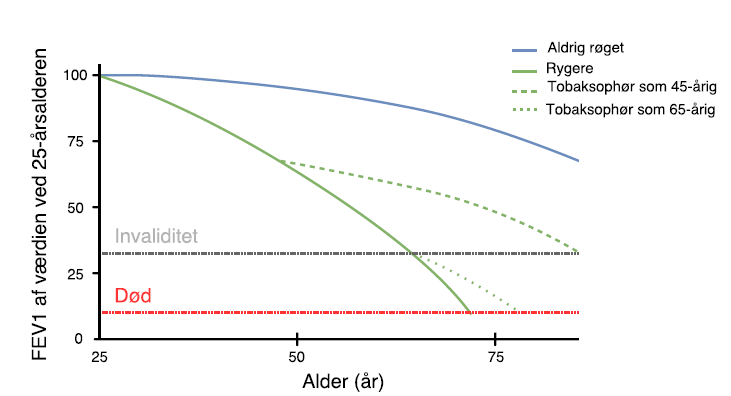
\includegraphics[width=0.5\textwidth]{figures/fletcher}
\caption{Fletcher-kurve som viser faldet af FEV1 over tid for henholdsvis rygere, ikke-rygere og rygere stoppet i $45$- og $65$-årsalderen.\cite{dsam2016}}
\label{fig:fletcher}
\end{figure} 

\noindent
Det ses af \autoref{fig:fletcher}, at rygning medvirker til et accelererende tab af FEV1. KOL-patienter, som har tobaksophør i $45$-års alderen, har udsigt til kortere levetid end patienter der aldrig har røget. Dog vil det accelerende tab af FEV1 mindskes til normal aftag ved tobaksophør.\cite{dsam2016}

Det anbefales, at patienter som kategoriseres til stadie $3$ eller derover i MRC-skalaen, udfører fysisk aktivitet og patienter med en BMI under $ 20$ bør desuden deltage i ernæringsrådgivning. 

Patienter med sekretproblemer tilbydes desuden continous positive airway pressure (CPAP) eller positive expiratory pressure (PEP-fløjte) og bronkodilaterende inhalationsbehandling efter behov og graden af KOL. Yderligere kan antiinflammatorisk behandling gives til patienter med hyppige eksacerbationer. \cite{Basisbogen2016}
 
 
\subsection{Prognose}
KOL-patienter med eksacerbationer har efter indlæggelse en dødelighed på næsten $10$~$\%$ i løbet af den første måned. Dødeligheden ligger på omkring $64$ per $100.000$ per år for mænd og $54$ per $100.000$ per år for kvinder.
Udviklingen, hvormed sygdommen progredierer for KOL-patienter er specielt afhængig af, om patienten ophører med rygning og/eller eksponering til den udløsende faktor, og det er derfor vigtigt at få en tidlig diagnosticering, således at patienten hurtigt kan få hjælp og dermed få så god en prognose som muligt. \cite{dsam2016}
Derudover har et studie vist, at KOL-patienter, der er i stadie $4$ i GOLD-klassificeringen, har lav funktionalitet og livskvalitet, som bliver værre med tiden og ved fremkomst af flere symptomer til sygdommen. \cite{Habraken2011}

